\section{Overview}
\begin{figure*}[t]
    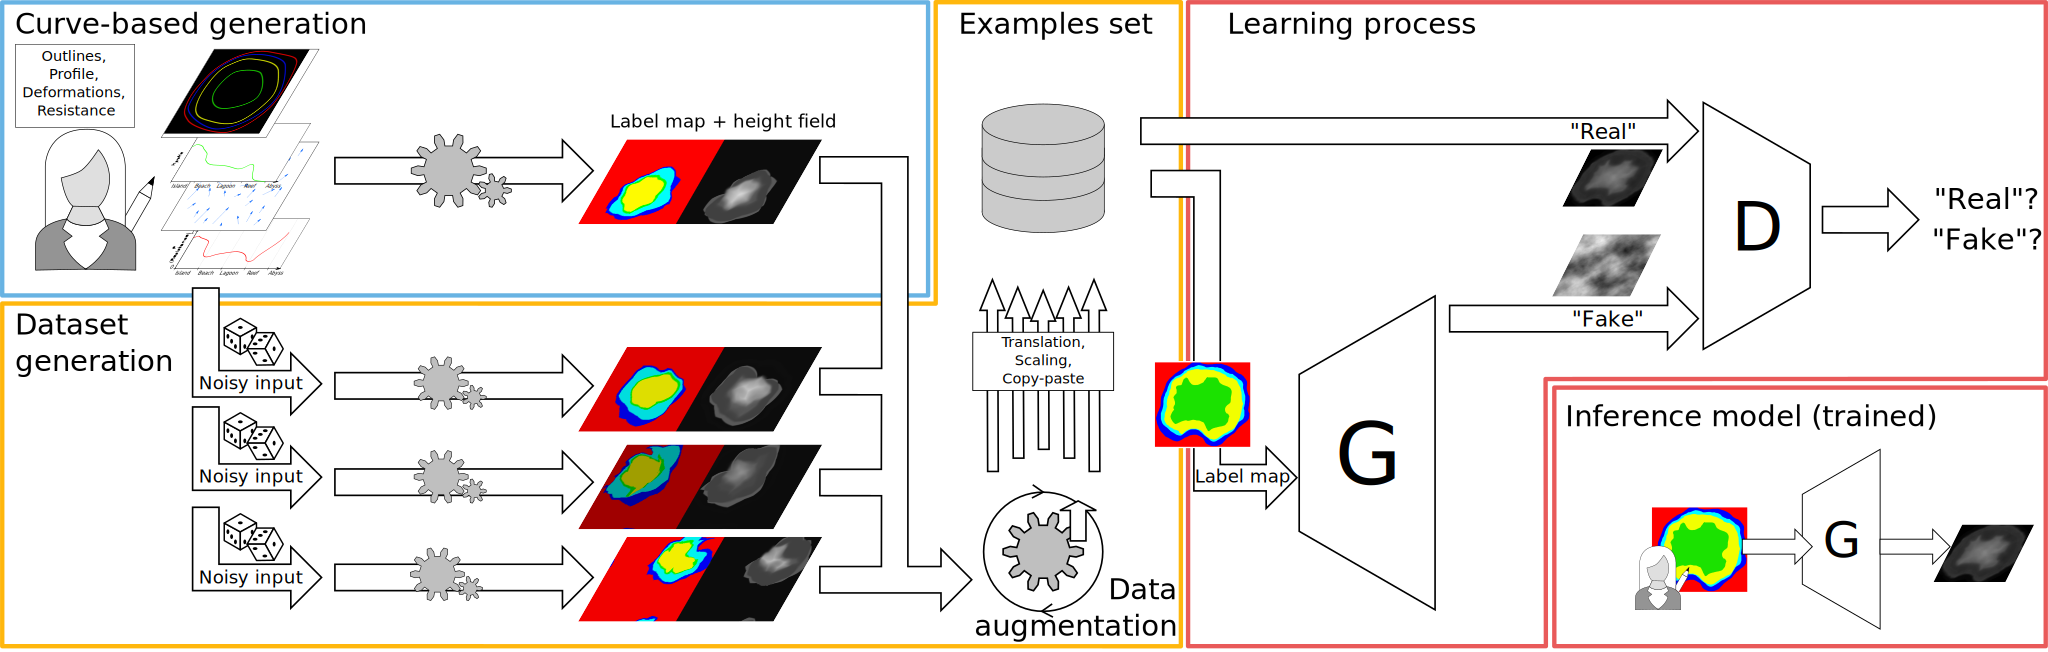
\includegraphics[]{pipeline_full.pdf}
    \vspace{-1em}
    \caption{Our pipeline first prompts the user to create single pairs of coral reef island height fields and label maps using our proposed curve-based modeling algorithm (\cref{sec:coral-island_example-generation}). The same algorithm is applied multiple times on randomly altered versions of the user input to create a dataset, which we further enhance with data augmentation techniques (\cref{sec:coral-island_dataset-generation}). Finally, we train a conditional Generative Adversarial Network, which can then be used standalone to create height fields from labelled sketches (\cref{sec:coral-island_learning-based}). }
        % \caption{Overview of our synthetic coral island generation pipeline. The system combines two complementary data generation strategies, linked by the automatic production of samples: (1) Curve-based generation (top-left) uses user-defined outlines, elevation profiles, and deformation controls to create structured label maps and corresponding height fields. Noisy input generation (bottom-left) synthesizes diverse examples using the user inputs with slight randomization, which are then stored in an example set and enhanced via data augmentation (center), including translation, scaling, and copy-pasting. (2) These pairs of label maps and height fields are used to train a conditional Generative Adversarial Network (cGAN) (right), where the generator $G$ learns to produce height fields from label maps, and the discriminator $D$ distinguishes "real" from "fake" data (i.e. produced from the curve-based generation agains those network-generated). After training, the inference model can generate realistic coral island terrain from new label maps designed by the user.}
    % \caption{[CA ARRIVE!!] Our method is split in three interleaved stages: the generation process (\cref{sec:coral-island_example-generation}) which creates pairs of height fields and label maps of an island from sketches, the model training (\cref{sec:coral-island_cGAN-training}) which use a synthetic dataset from the previous stage to obtain a cGAN model that generates height fields from label maps to remove the constraints embedded in the initial generation process, and finally, the inference process (\cref{sec:coral-island_results}) uses the trained cGAN to generate the final height fields, including the coral generation process, automatically. }
    \label{fig:coral-island_pipeline}
\end{figure*}

Our method for procedural generation of coral reef islands is composed of two independent modeling techniques shown in \cref{fig:coral-island_pipeline}. A first curve-based algorithm  (top-left blue block, presented in \cref{sec:coral-island_example-generation}), parametrizes the surface of islands by a top-view sketch interface, describing the outlines of its constituent regions and a stroke-based wind field deforming them, as well as a profile-view sketch describing for each region its altitude and resistance to deformations. User inputs are given as 1D functions (altitude and resistance), a 1D polar function (island outlines) and a 2D vector field (wind field) as shown in \cref{fig:coral-island_wind-from-strokes-interaction}, which are convinient to randomize through the use of noise, but limit the user's freedom to model arbitrary shapes.

We propose a second learning-based generation algorithm (right red blocks \cref{fig:coral-island_pipeline}, developed in \cref{sec:coral-island_learning-based}), which trains a neural generator $G$ to transform a labelled image into a height field. Parallely, a discriminator $D$ is trained to distinguish height fields provided from the training set against height fields generated by $G$. This adversarial training strengthens the outputs of the generator, up to the point where we discard the discriminator and training data, only keeping the generation step (bottom-right). Users are then able to provide unseen label maps and obtain height fields as close as possible to the training dataset. This method for terrain modeling is poorly constrained, however requires a large amount of prior data in its training set, which is not available in our case.

We connect these two algorithms through a process of dataset generation (central orange block \cref{fig:coral-island_pipeline}, described in \cref{sec:coral-island_dataset-generation}) in order to enforce the benefits of each while reducing their limitations. Given the initial curve-based user inputs, we create a dataset composed of similar samples processed by our first algorithm, rasterized into a 2D image of the parametrized regions, and paired with the resulting height field. We then greatly increase the size of the dataset by employing various data augmentation techniques such as translations, scaling and copy-pasting of multiple islands in a single sample. We then obtain a dataset large enough for training our cGAN and enable users to procedurally create coral reef islands with a high level of control.


\begin{figure}[tb]
    \centering
    \includegraphics[width = 0.9 \linewidth]{user_interaction_generation.png}
    \caption{The user can interact directly on the island by editing the different canvases in any order. This UI shows, from left to right, the top-view sketch with the different outlines of each regions, the profile-view sketch with the outlines represented by dotted lines, the wind velocity sketch drawn with strokes (last stroke is visible), and the resistance function showing here a high resistance at the top of the island and on the front reef.}
    \label{fig:coral-island_wind-from-strokes-interaction}
\end{figure}

% Our method for generating coral reef islands combines user-driven sketching, procedural techniques, and deep learning to create realistic and varied island terrains (\cref{fig:coral-island_pipeline}). 

% The pipeline consists of two distinct phases: a procedural data-generation phase and a deep-learning-driven inference phase. 

% \subsection{Procedural generation phase}
% \label{sec:coral-island_proc-phase}

% In the initial procedural phase, the user sketches key island features from two complementary viewpoints: a top view, defining the horizontal layout of island features (island boundaries, beach width, lagoon areas, coral reefs), and a profile view, specifying the vertical elevation profile from island center to ocean (\cref{sec:coral-island_generation-initial}).

% Additionally, users can sketch a wind deformation map, enabling simulation of natural erosion patterns caused by wind and waves (\cref{sec:coral-island_wind-deformation}).

% From these sketches, the procedural system generates a synthetic island terrain with the keep-up stategy of coral reefs (\cref{sec:coral-island_coral-reef}) and a corresponding semantic label map, where each pixel indicates its region type (island, beach, lagoon, reef, abyss) (\cref{sec:coral-island_procedural-output}).




% \paragraph{User interaction}
% \label{sec:coral-island_description-UI}

% \begin{figure}
%     \centering
%     \includegraphics[width = 0.9 \linewidth]{user_interaction_generation.png}
%     \caption{The user can interact directly on the island by editing the different canvases in no specific order. This UI shows, from left to right, the top-view sketch with the different outlines of each regions, the profile-view sketch with the outlines represented in dotted lines, the wind velocity sketch drawn with strokes (last stroke is visible), and the resistance function showing here a high resistance at the top of the island and on the front reef.}
%     \label{fig:coral-island_wind-from-strokes-interaction}
% \end{figure}

% As users draw the top-view and profile-view sketches, the system provides real-time feedback on the resulting terrain. The top-view sketch influences the horizontal layout of the island, while the profile-view sketch defines its vertical structure. These sketches can be adjusted independently, allowing the user to fine-tune both the outline and elevation of the island.

% While sketching the basic shape, users can apply wind deformation strokes to modify the island's features further. These strokes represent wind and wave influences, distorting the island's shape to introduce more natural, non-radial features such as indentations along the coastline, variable lagoon shapes, or concave formations. The system automatically applies these deformations, providing real-time feedback as the user interacts with the terrain.

% This interactive process, combining sketches and wind deformation, allows users to quickly iterate on their designs, refining the terrain to meet specific aesthetic or functional goals.

% \subsection{Learning-based generation phase}
% \label{sec:coral-island_cGAN-phase}

% We repeat this procedural generation process multiple times with varied parameters (different shapes, scales, subsidence levels, and wind patterns) to create a large synthetic dataset (\cref{sec:coral-island_dataset-generation}). Each dataset entry consists of a label map paired with its procedurally generated terrain height field. Data augmentation is applied to the generated pairs to reduce the impact of the constraints induced from the procedural method (\cref{sec:coral-island_data-augmentation}).

% We use this dataset to train a Conditional Generative Adversarial Network (cGAN), specifically the pix2pix architecture, capable of translating label semantic maps into realistic terrain height fields (\cref{sec:coral-island_dataset-generation}).

% After training, the procedural step becomes unnecessary. To generate new island terrains, the user only needs to provide a label semantic map as input to the trained cGAN. The cGAN then synthesizes realistic island elevation details directly, capturing learned geological and geomorphological patterns from the synthetic training data (\cref{sec:coral-island_results}).

% \paragraph{User interaction}
% \label{sec:coral-island_cGAN-phase-interaction}

% Thus, the trained cGAN provides a user-friendly interface: users draw or edit simple label maps (regions) to rapidly generate diverse, geologically plausible coral reef island terrains, incorporating realistic features such as smooth transitions between regions, detailed coral reef structures, and naturally varied shapes free from procedural constraints.

% \midConclusion

% This combined procedural-and-learning approach provides a simple, flexible, and powerful tool for island terrain generation, enabling users to intuitively generate realistic and diverse coral reef islands aligned with real-world geological and biological processes such as volcanic subsidence, coral reef growth, and wind-driven erosion.